\chapter{考察}
ここでは本研究が行った実験とその評価についての考察を述べる.
\section{精度の考察}
画面全体を検出した場合の表\tabref{tab:mAP_fig_noweght}と\tabref{tab:mAP_fig}を比較する.
2つの表を比較した際に,大きな違いはFPである.実装したDepth2Jamは画面中央部分のみを検出するように改良したためFPがどの動画においても0という結果になっているが,画面全体を検出する場合ではFPが最大で29まで増加している.
画面両端の1/3部分を検出しないようにした結果,Depth2Jamの正確性が向上したことがこの比較でわかる.
次に,映像5における2つの結果を比較した際に,\tabref{tab:mAP_fig_noweght}においてはF値が0.82と\tabref{tab:mAP_fig}におけるF値の0.33より大幅に上昇している.

\subsection{誤検出}
まず,\ref{sec:exp1}における誤検出の例とその原因についての考察を述べる.
\tabref{tab:exp3_fig}において,映像1においては誤推定されたフレームは存在しないが,映像2においては渋滞ではないのに渋滞だと誤推定されたフレームが存在する.
誤推定されたフレームの例を\figref{fig:mov2miss01}と\figref{fig:mov2miss02}に示す.

% ---------------------------------
\begin{figure}[htbp]
  \begin{minipage}{0.5\hsize}
   \begin{center}
    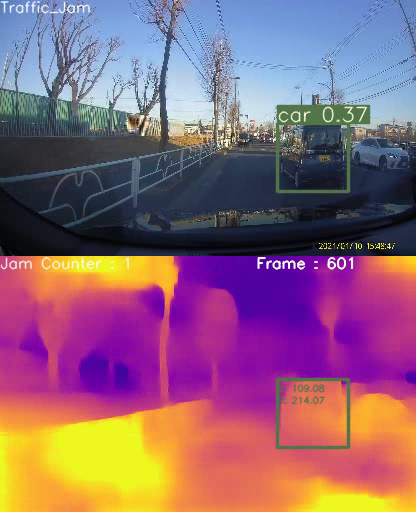
\includegraphics[width=7cm]{figs/mov2miss/miss01.png}
   \end{center}
   \caption{誤検出の例1}
   \label{fig:mov2miss01}
  \end{minipage}
  \begin{minipage}{0.5\hsize}
  \begin{center}
   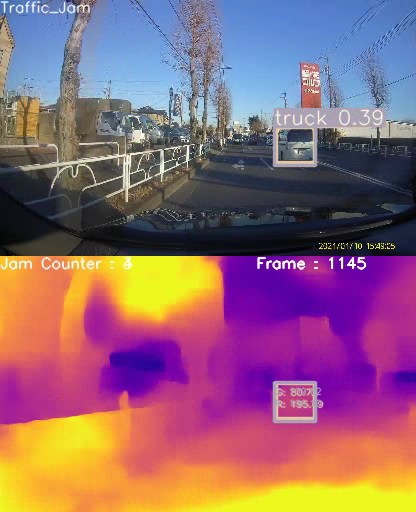
\includegraphics[width=7cm]{figs/mov2miss/miss02.png}
  \end{center}
   \caption{誤検出の例2}
   \label{fig:mov2miss02}
  \end{minipage}
 \end{figure}
% ---------------------------------

どちらのフレーム画像においても検出された自動車が中央に寄っており,かつ検出されたBBOXにおける平均G値が100を超えてしまっているので渋滞だと判断してしまっていることがわかる.
実装したDepth2Jamシステムにおいては,画面左右1/3における自動車の検出がされないようにしているが,この検出除外処理は,検出されたBBOXにおける2つのX軸の値のうち,左側つまり小さい方の値のX軸が画面の左右1/3の範囲に含まれる場合に発生する.
このフレームではそのX軸の値が中央1/3の範囲に含まれているためこのような結果になったのだと思われる.
より精度を向上させるために,BBOXにおけるX軸の値のうち,右側つまり値の大きい方のX軸に対しても追加で検出除外処理を設ける必要があると考えられる.

\newpage
\subsection{FNに関する考察}
ここでは,\tabref{tab:mAP_fig}におけるFNに関する考察について述べる.
映像1と映像2に関しては渋滞しているフレームは存在しないのでFNの値も0となっているが,映像3~5および総合においてはFNの値が目立つ.
FNはシステムが渋滞でないと判断したが,実際には渋滞していたフレームであり,現実では信号や渋滞等で自動車が動いていないのにシステムが渋滞だと判断できていなかったフレームである.
そのフレームの例を\figref{fig:fn01}と\figref{fig:fn02}に示す.

% ---------------------------------
\begin{figure}[htbp]
  \begin{minipage}{0.5\hsize}
   \begin{center}
    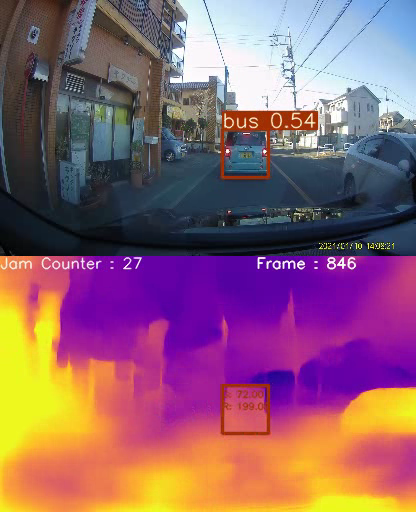
\includegraphics[width=7cm]{figs/consider/fn01.png}
   \end{center}
   \caption{FNの例1}
   \label{fig:fn01}
  \end{minipage}
  \begin{minipage}{0.5\hsize}
  \begin{center}
   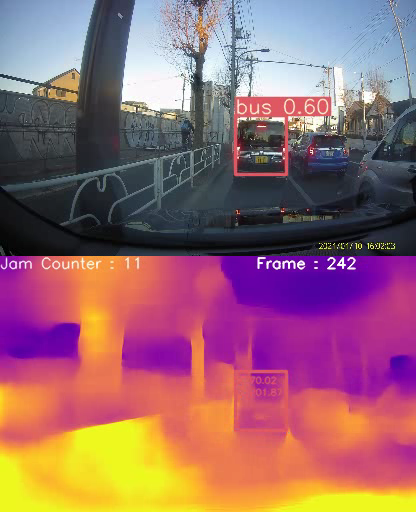
\includegraphics[width=7cm]{figs/consider/fn02.png}
  \end{center}
   \caption{FNの例2}
   \label{fig:fn02}
  \end{minipage}
 \end{figure}
% ---------------------------------

どちらの例も先行車が停車しており,ドライブレコーダーを搭載した自動車も停車している状況である.
そして,検出されたBBOXにおいて,G値の値は70程度となっており,渋滞と判断されていない.
考えられる原因としてはドライバーが車間距離に余裕を持って停車しているため,G値が相対的に小さくなってしまっていることにあると考えられる.
車間距離に余裕を持って停車することは本来推奨される運転のため,余裕を持って車間距離をとっている場合でも渋滞だと推定できる手法を取る必要がある.

